\documentclass[graphics]{beamer}

\usepackage{graphicx}
\usepackage{verbatim}
\usepackage{wrapfig}
\useoutertheme{shadow}
%\usecolortheme{orchid}
\usecolortheme{seahorse}


% math commands
\newcommand{\be}{\begin{eqnarray}}
\newcommand{\ee}{\end{eqnarray}}
\newcommand{\beq}{\begin{equation}}
\newcommand{\eeq}{\end{equation}}
\def\simless{\mathbin{\lower 3pt\hbox
      {$\rlap{\raise 5pt\hbox{$\char'074$}}\mathchar"7218$}}}
\def\simgreat{\mathbin{\lower 3pt\hbox
      {$\rlap{\raise 5pt\hbox{$\char'076$}}\mathchar"7218$}}} %> or of order

% variables

\def\toonscale{0.45}
\def\mboxy#1{\mbox{\small #1}}


\begin{comment}
\AtBeginSection[]{
  \frame{
    \frametitle{Outline}
    \tableofcontents[currentsection]
  }
}
\end{comment}

\title{Neutrino Torques
}
\subtitle{}
\author[U. Pen]{\textcolor{green}{H. Yu, X. Wang}
\\[8mm] 
}
\date{October 26, 2018}


\begin{document}

\frame{
\begin{picture}(320,250)
\put(-50,-130){
\includegraphics[width=5.5in]{Figures/delta_nu_sim.pdf}}
\end{picture}
\vspace{-3in}
\titlepage
}

%\section*{Introduction}
\section{Cosmological Neutrino Clustering}

\begin{comment}
  \subsection{Outline}

  \frame{
    \frametitle{Outline}
    \tableofcontents
  }
\end{comment}

  \frame{
\vspace{-0.5in}
    \frametitle{Neutrinos}
    \begin{itemize}
        \item minimum mass 0.05 eV: $\Omega_\nu \sim 10^{-3} \ll \Omega_b$
        \item most massive neutrino non-relativistic today, affects LSS
        \item normal or inverted hierarchy?
        \item cosmological probes: how to disentangle such a small
          effect
        \item statistics not main problem: SDSS $1/\sqrt{n} \sim 10^{-3}$
%          \vspace{-0.15in}
    \end{itemize}
  }
  \frame{
    \frametitle{Observables}
    \begin{itemize}
        \item CMB, gravitational lensing: 2-D projection
        \item galaxies: 3-D biased displacement field
        \item Monger-Ampere equation/solution
        \item ideally measure 2 fields, infer 2 fields: CDM, neutrinos (HDM)
    \end{itemize}
\vspace{-0.1in}\hspace{.3in}
\includegraphics[width=2.2in]{Figures/th2photo.jpg}
}
  \frame{
    \frametitle{Movie}
    {\tt http://cita.utoronto.ca/\~\,haoran/thnu/movie.html}
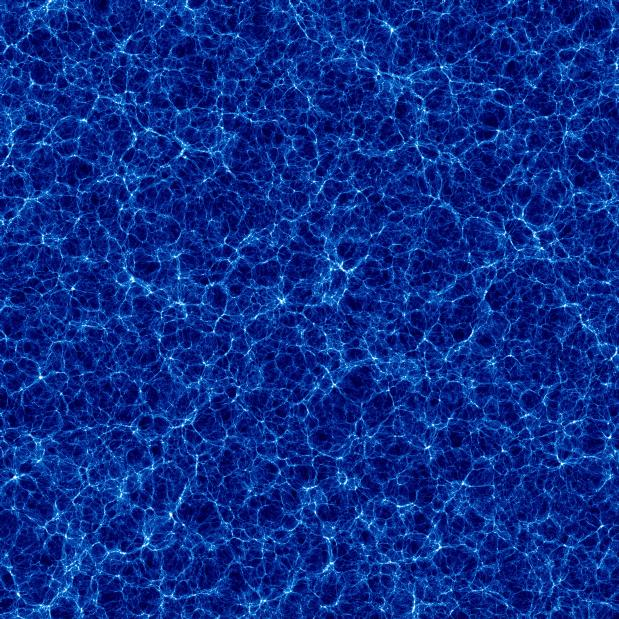
\includegraphics[width=4.2in]{Figures/thnucdmlowres.jpg}
}
  \frame{
    \frametitle{Differential clustering}
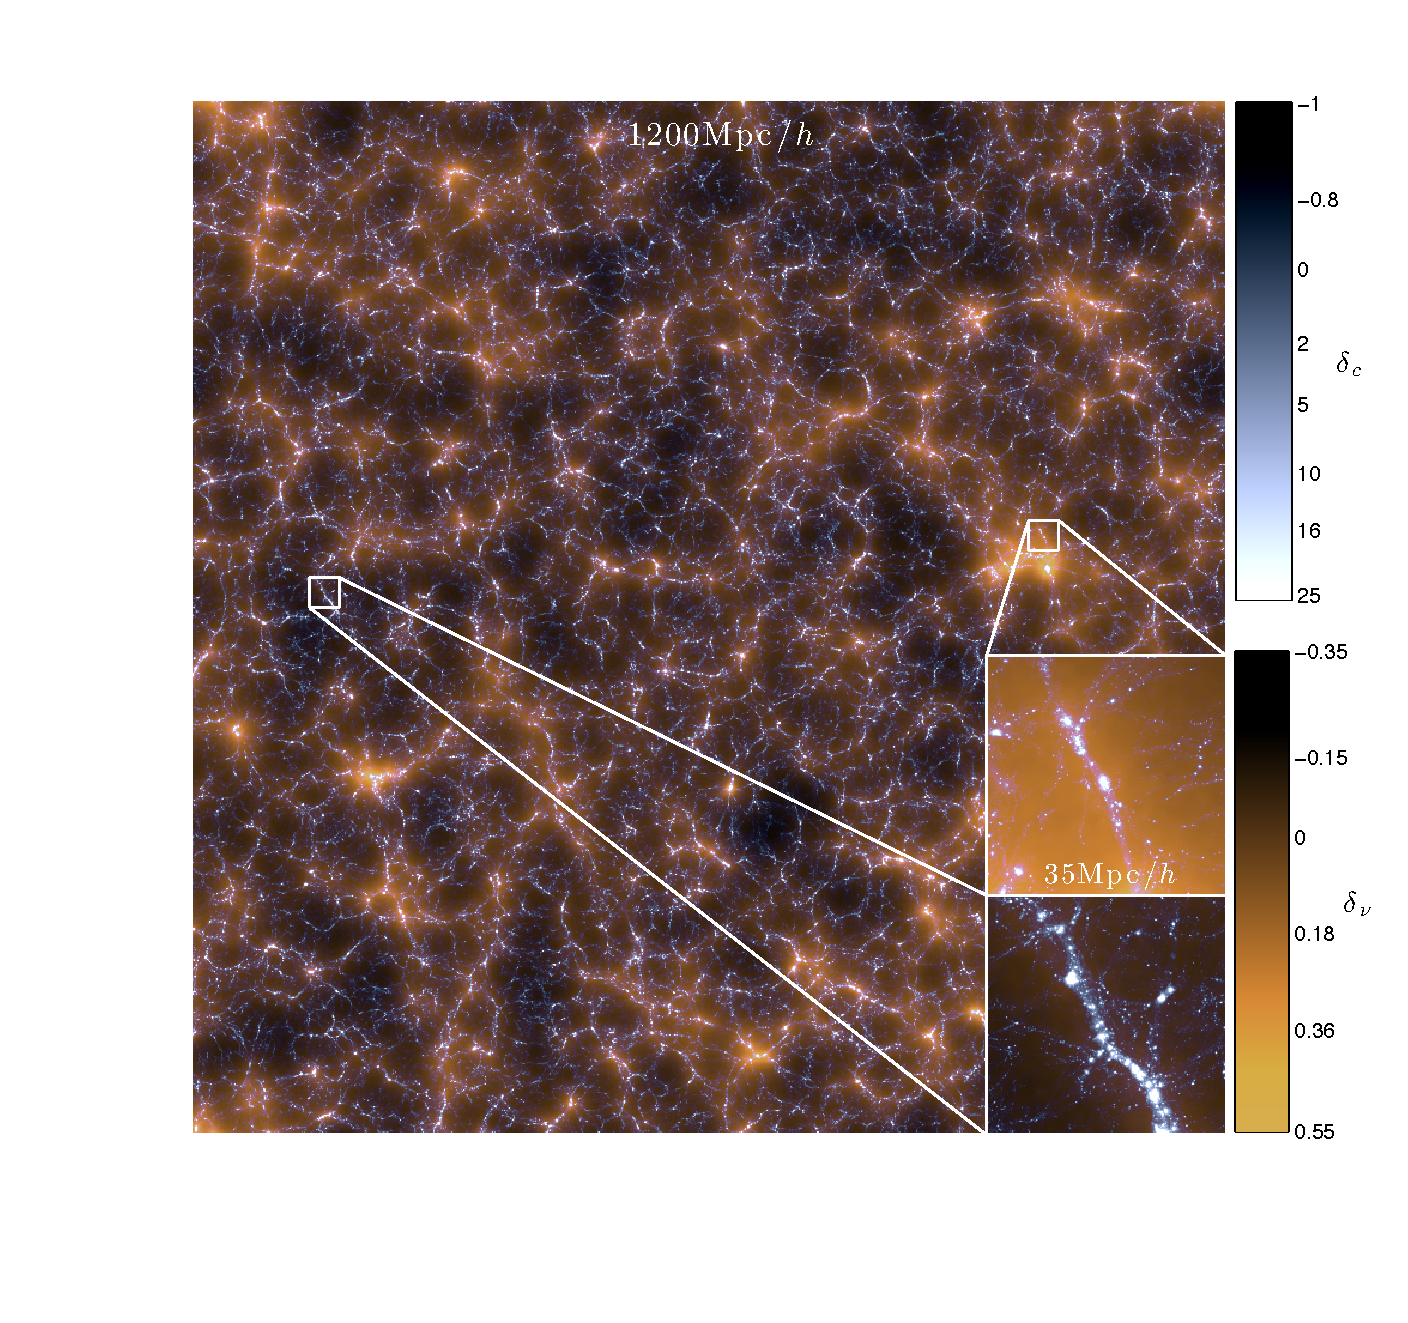
\includegraphics[width=3.5in]{Figures/cnudiff.pdf}
}
  \frame{
    \frametitle{Halo Reconstructed $\nu$ field}
%\vspace{0.5in} 
left: sim, right: wiener halo reconstructed
\vspace{-0.9in}
\hspace{-0.6in}
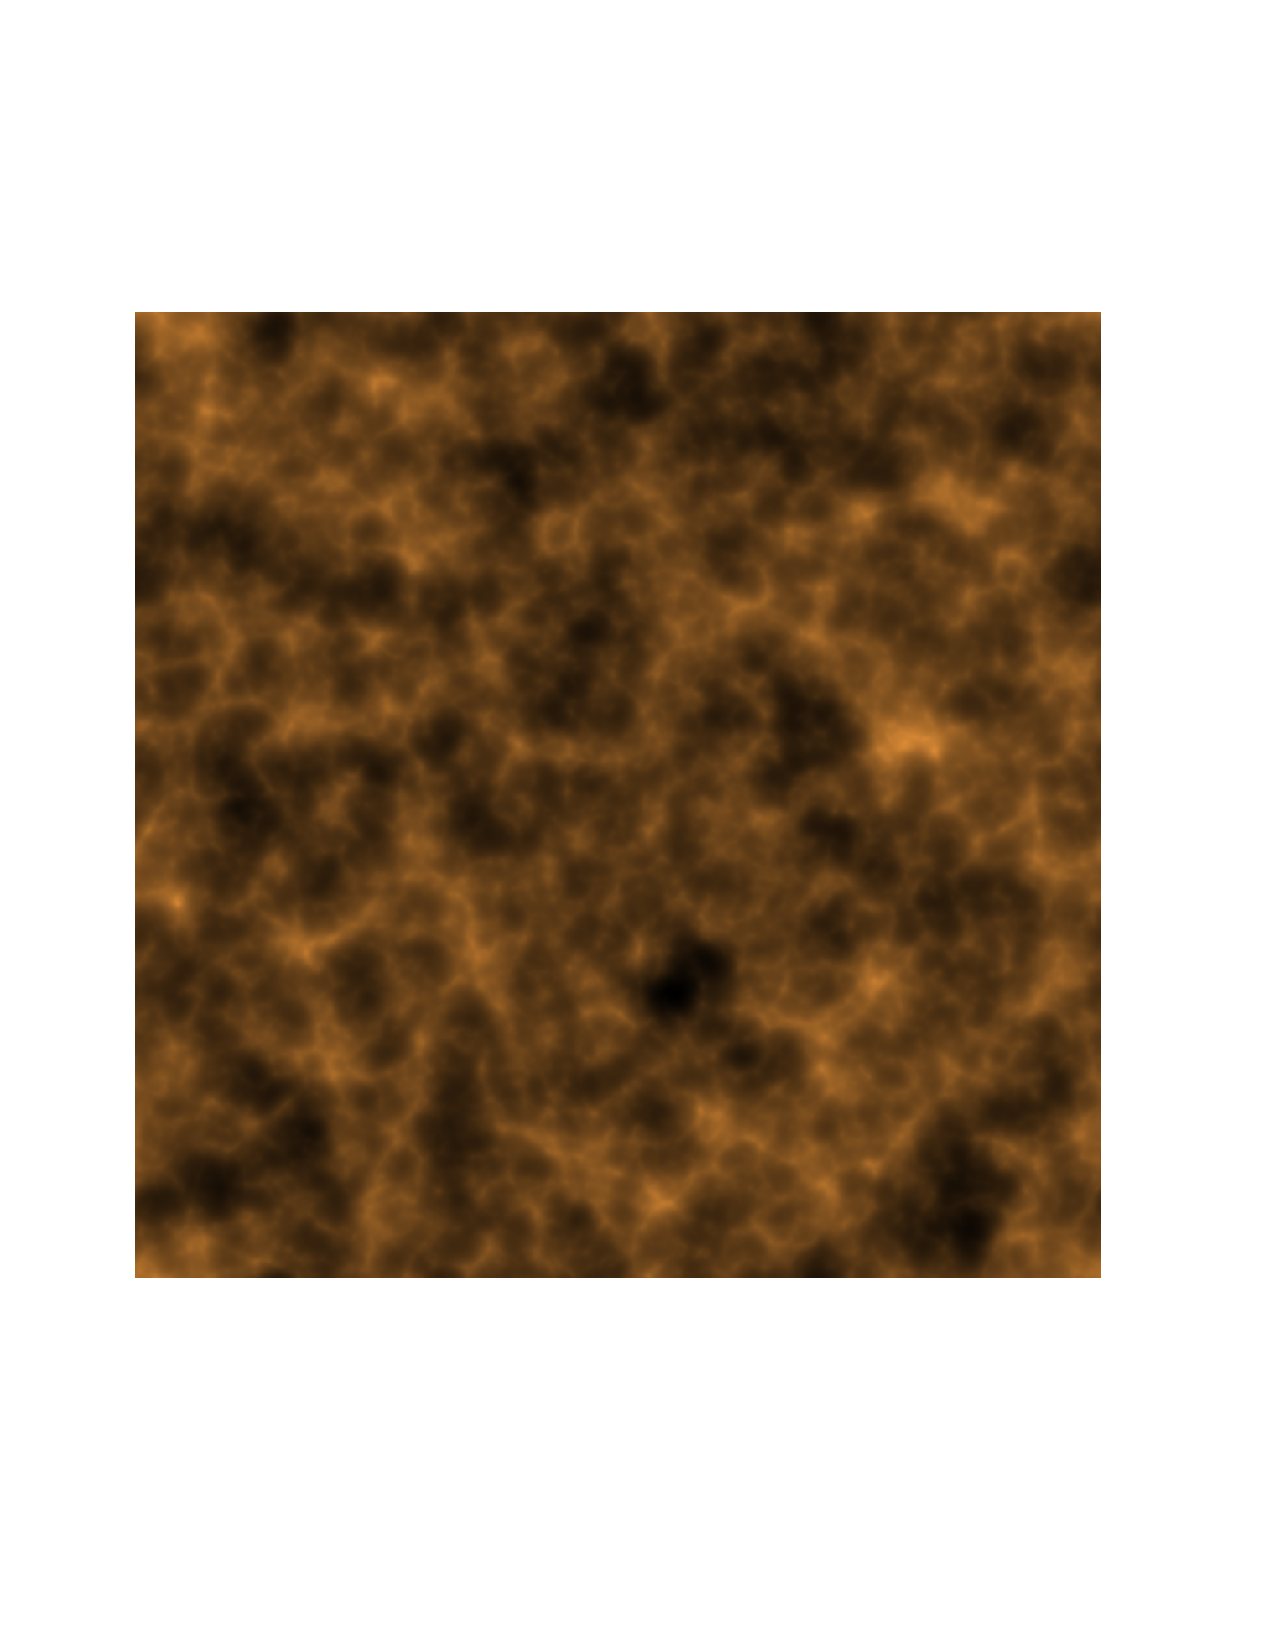
\includegraphics[width=2.7in]{Figures/delta_nu_reco_wien.pdf}
\hspace{-0.6in}\includegraphics[width=2.7in]{Figures/delta_nu_sim.pdf}
}
  \frame{
    \frametitle{$\nu$ -Condensation}
\vspace{-1.0in}
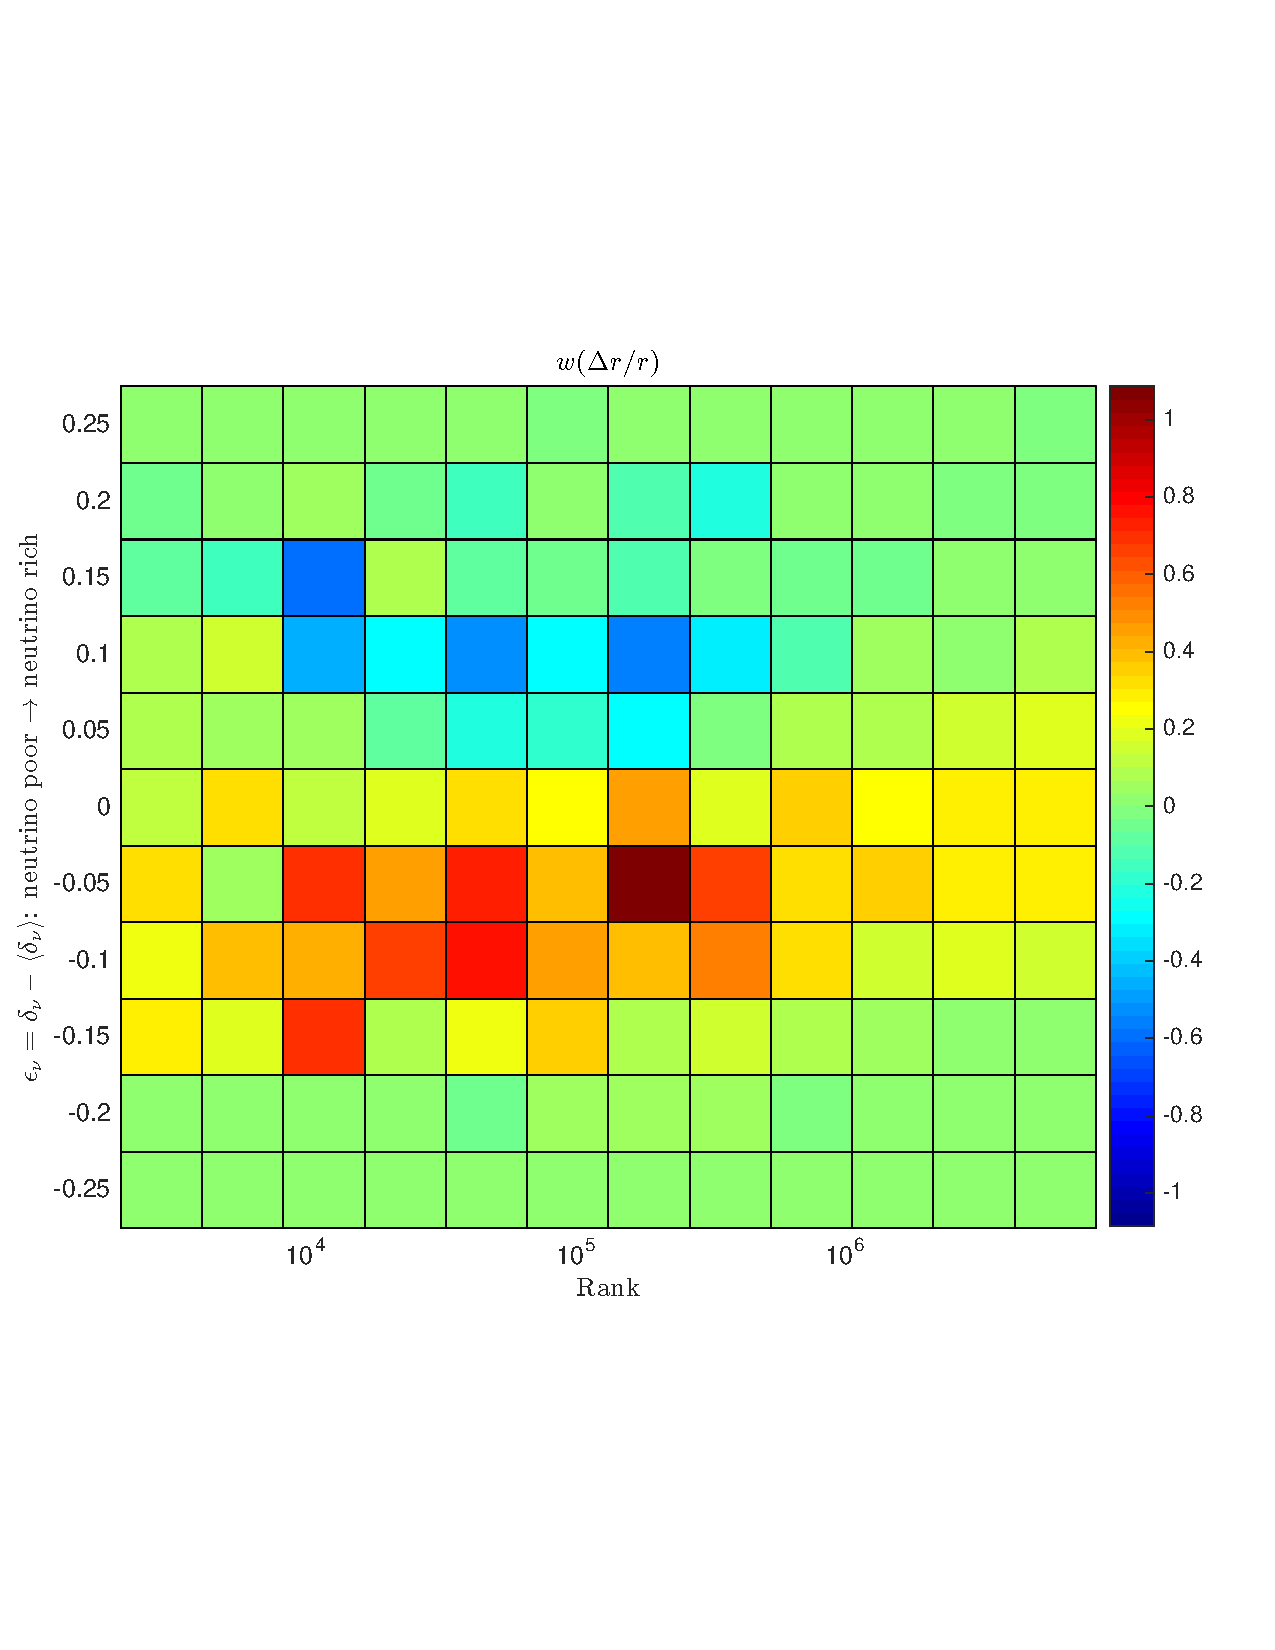
\includegraphics[width=4.0in]{Figures/color.pdf}
}
  \frame{
    \frametitle{$\nu$ -bias}
\vspace{-1.0in}
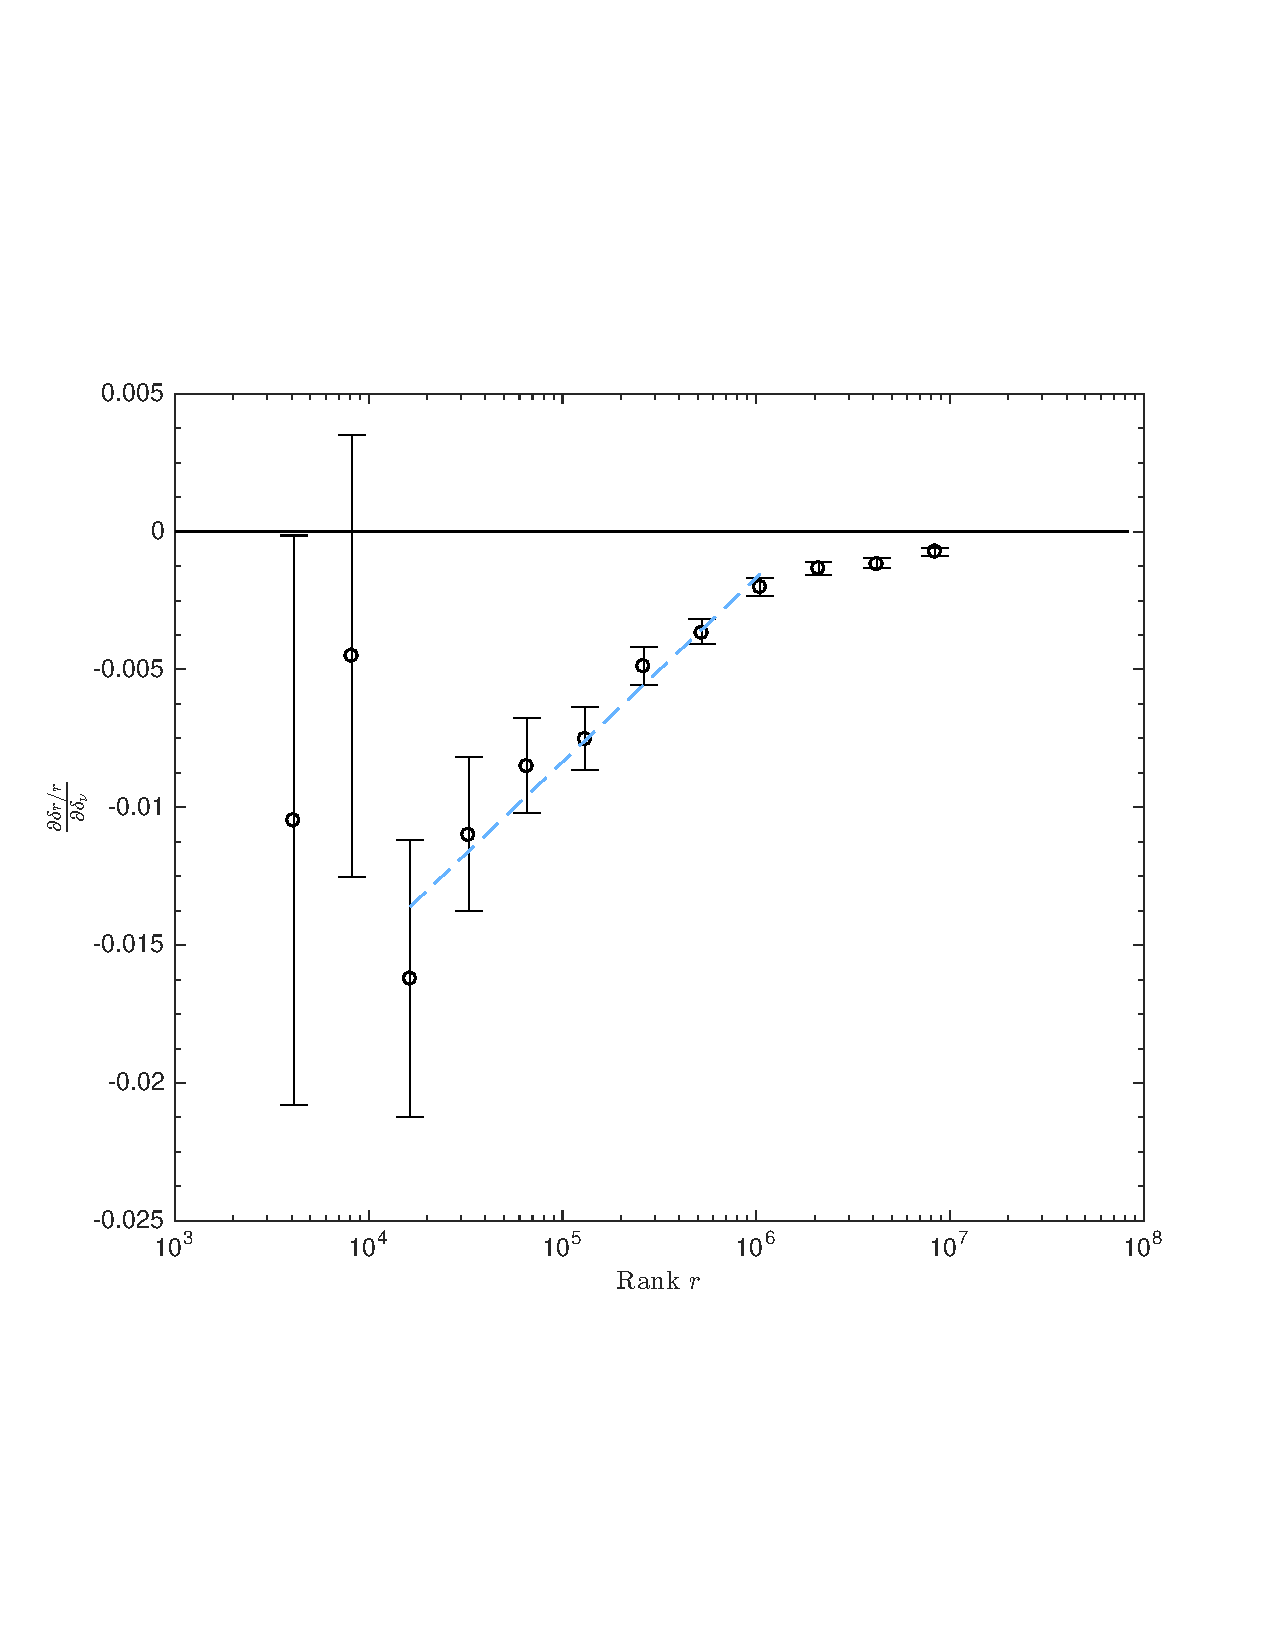
\includegraphics[width=4.0in]{Figures/slope_fit}
}
  \frame{
    \frametitle{Mass rank}
\vspace{-0.9in}
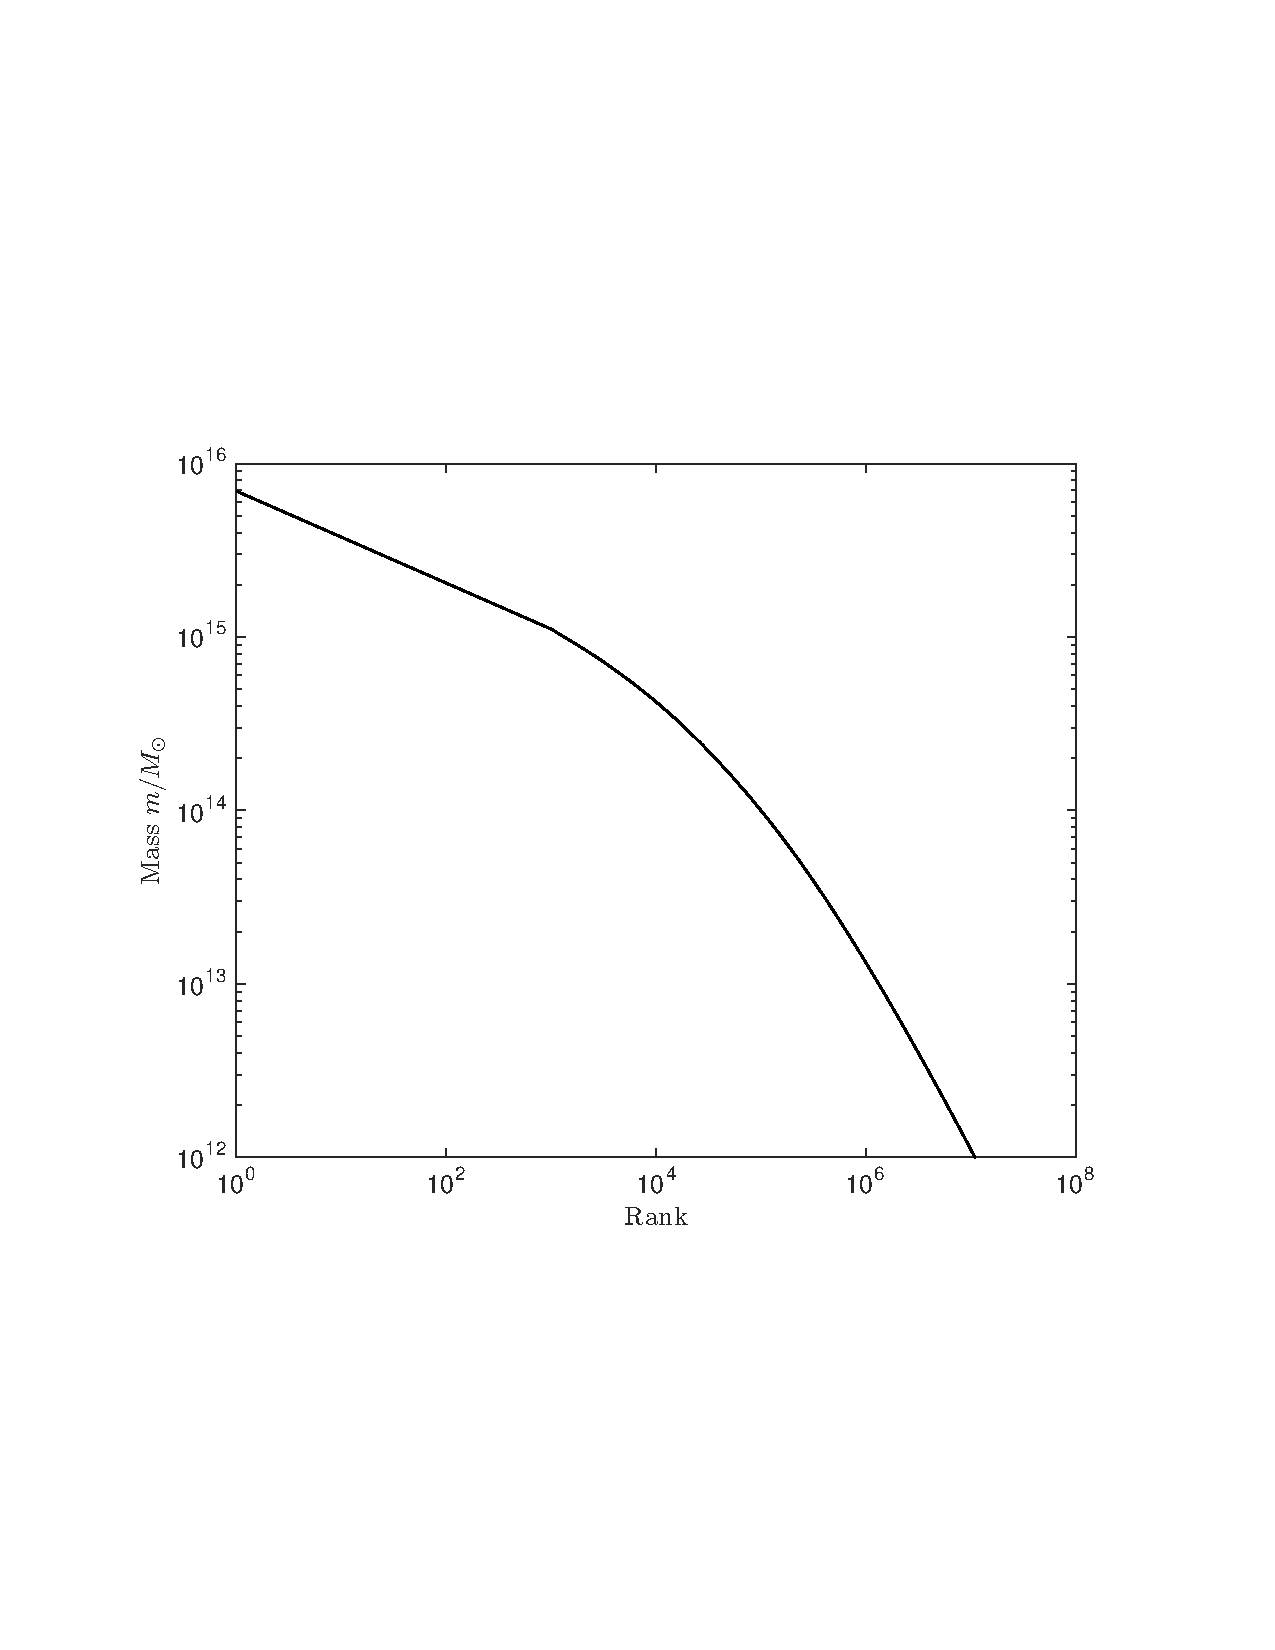
\includegraphics[width=4.0in]{Figures/HMF.pdf}
}

\frame{
\vspace{-0.5in}
    \frametitle{1-D bijective potential isomass coordinate}
    \begin{itemize}
        \item McQuinn\&White 2016
        \item unique mass coordinate
        \item closest non-parametric reconstruction (Zhu et al 2016)
     \end{itemize}
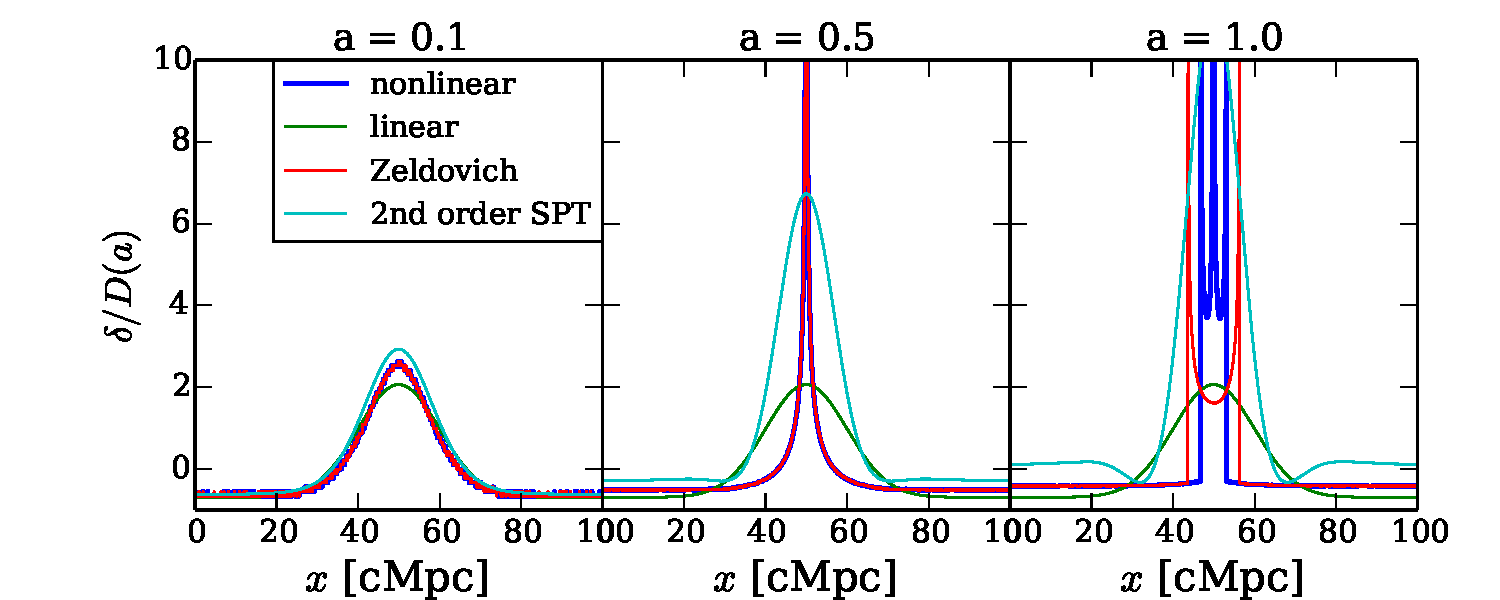
\includegraphics[width=4.21in]{Figures/gaussian_pert.pdf}  
  }
\frame{
    \frametitle{3-D: E-mode}
%\vspace{-0.5in}
\hspace{-0.2in}\includegraphics[width=2.3in]{Figures/nonlinear.png}  
\vspace{0.15in}\includegraphics[width=2.21in]{Figures/reconstructed.png}  

(from Yu et al 2016, 1610.7112)
  }

\frame{
    \frametitle{Lagrangian coordinates}
\center{\includegraphics[width=4.3in]{Figures/delta_reco_raw.pdf}  }
  }

  \frame{
    \frametitle{Coordinate freedom}
\begin{eqnarray}
{\rm potential\ deformation\ \ \ \ \ }  x^i &=& \xi^\mu \delta^i_\mu + \frac{\partial \phi}{\partial
    \xi^\mu}\delta^{i\mu}\nonumber\\
{\rm dreibein\ \ \ \ \ \  } e^i_\mu &\equiv& \partial x^i / \partial \xi ^ \mu \nonumber\\
 {\rm volume\  element\ \ \ \ }\sqrt{g} &\equiv& \mathrm{det}\left| e^i_\mu\right|\nonumber\\
{\rm mass\ coordinate \ \ \ \ \ }    \rho \sqrt{g}&=&\mathrm{Const.}\nonumber\\
    \partial _\mu (\rho \sqrt{g} e^\mu _i \delta^{i\nu}
    \partial_\nu \dot{\phi})&=&\langle\rho\rangle-\rho \sqrt{g}
\label{eqn:dif}
\end{eqnarray}
Solve diffusion eqn (\ref{eqn:dif}) using multigrid (Pen 1995)
}

  \frame{
    \frametitle{Multigrid solution}
\vspace{-0.7in}\center{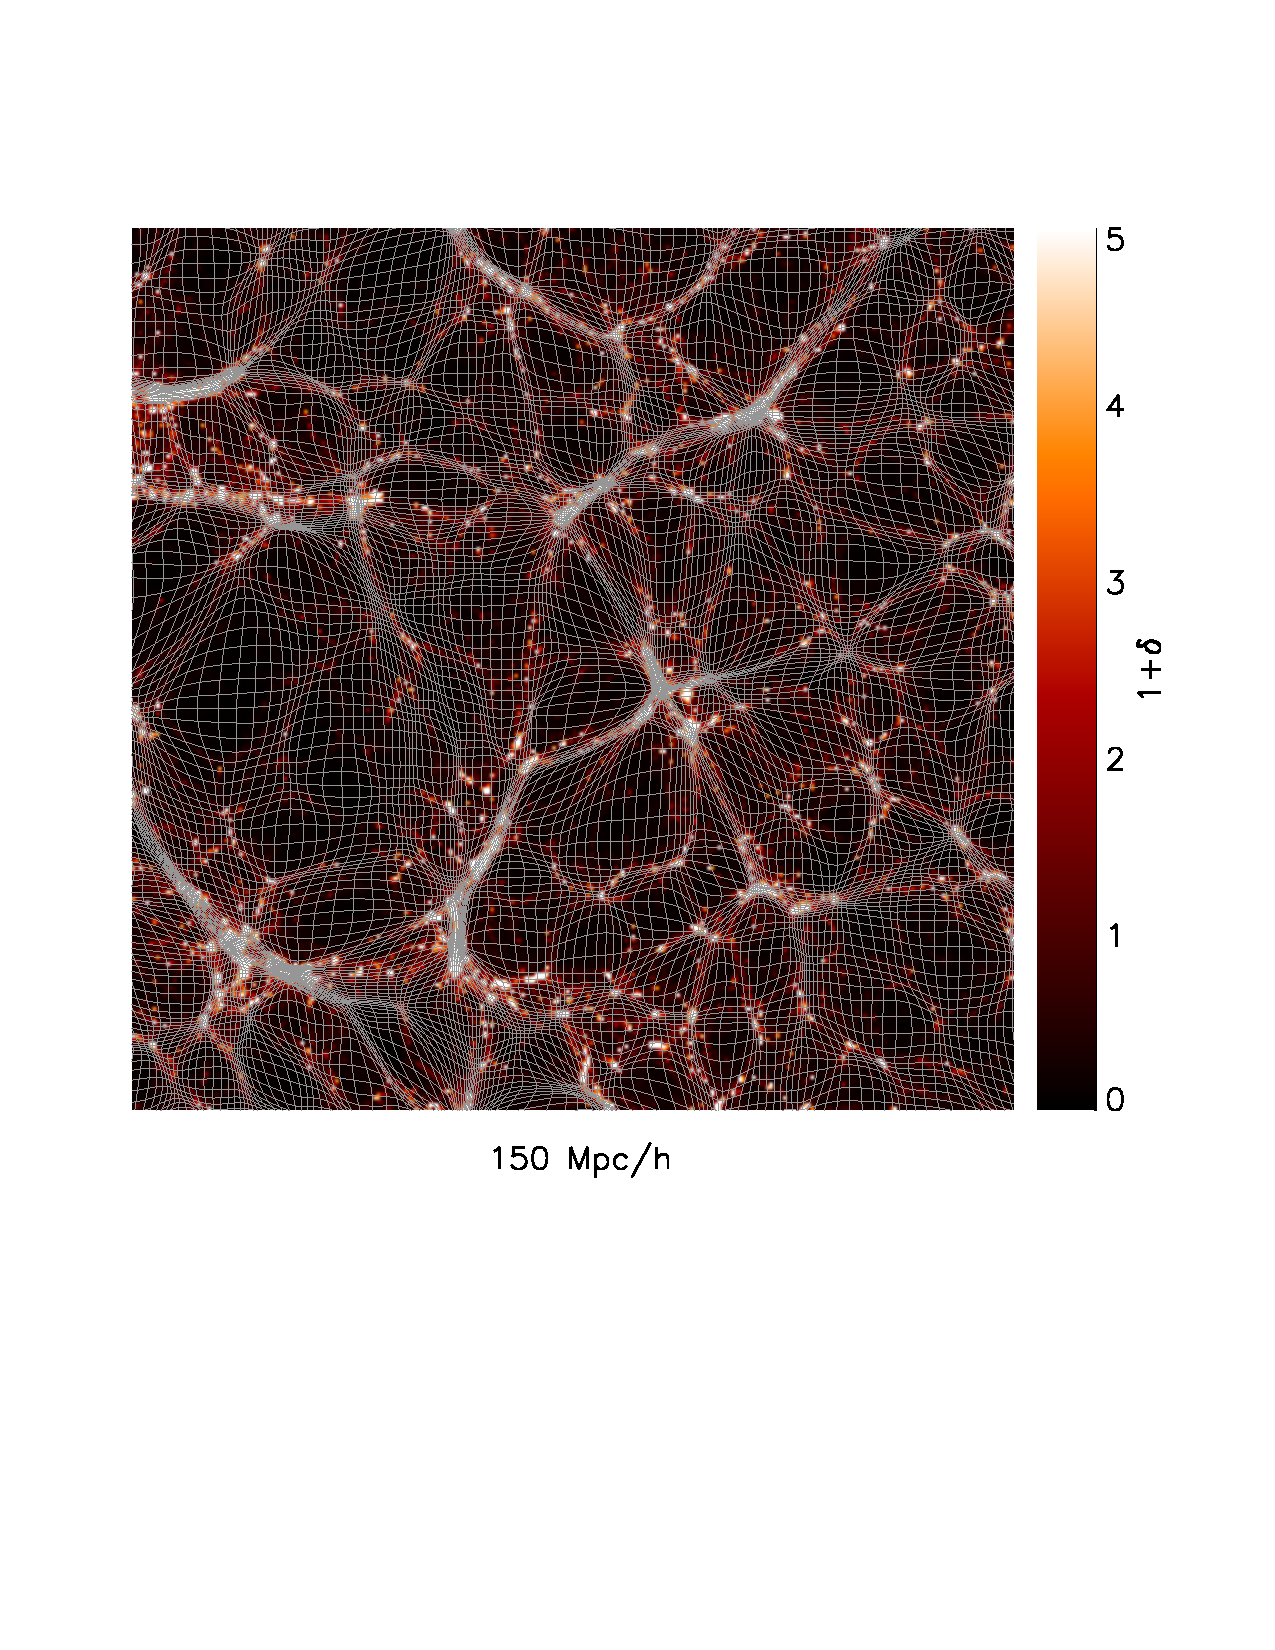
\includegraphics[width=4.0in]{Figures/map0512-0128_i1500_xz222.pdf}}
Zhu et al 1610.09638
}
  \frame{
    \frametitle{Redshift space}
\vspace{-0.7in}\center{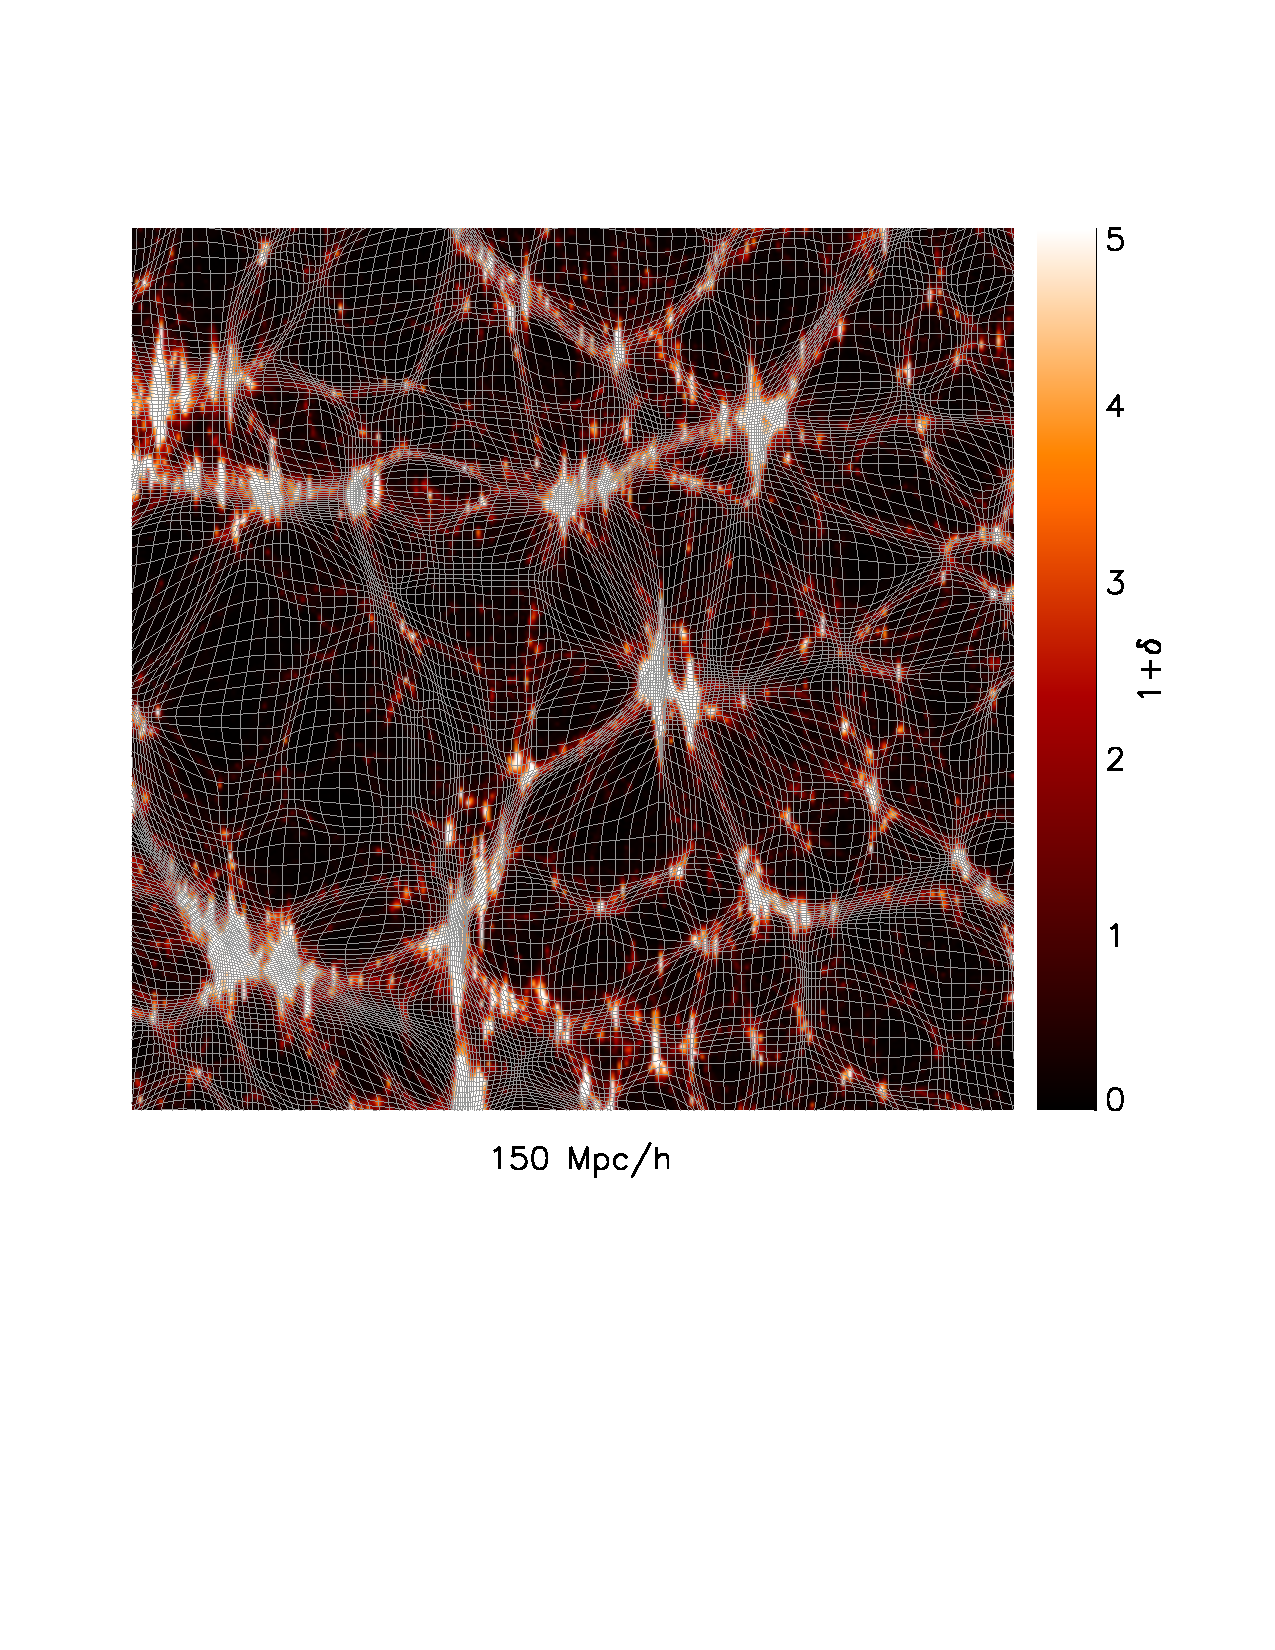
\includegraphics[width=4.0in]{Figures/map0512-0128_i0900_xz222_rsd3.pdf}}
Zhu et al 1610.09638
}

  \frame{
    \frametitle{Low noise limit}
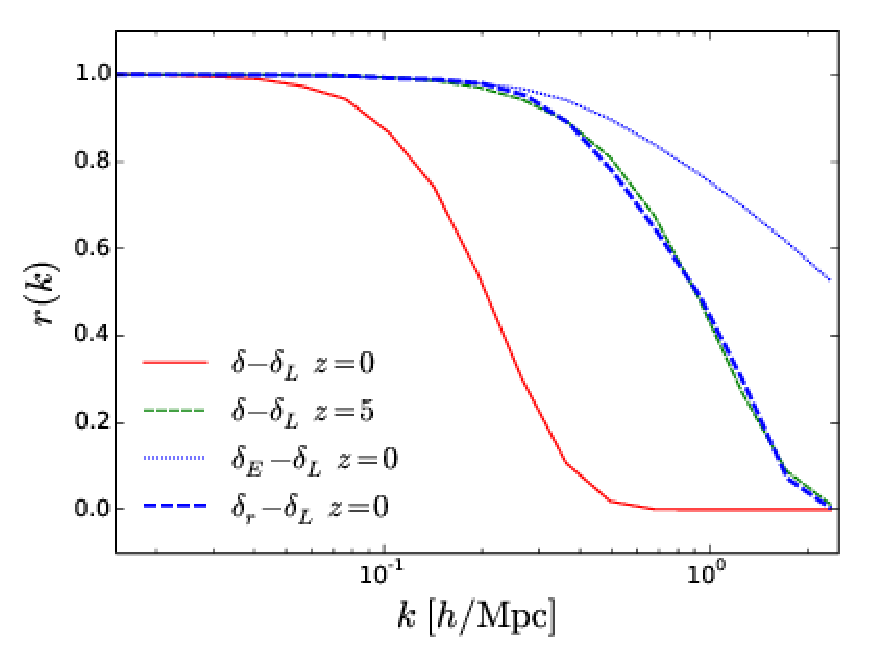
\includegraphics[width=3.4in]{Figures/rk.pdf}
}
  \frame{
    \frametitle{BAO}
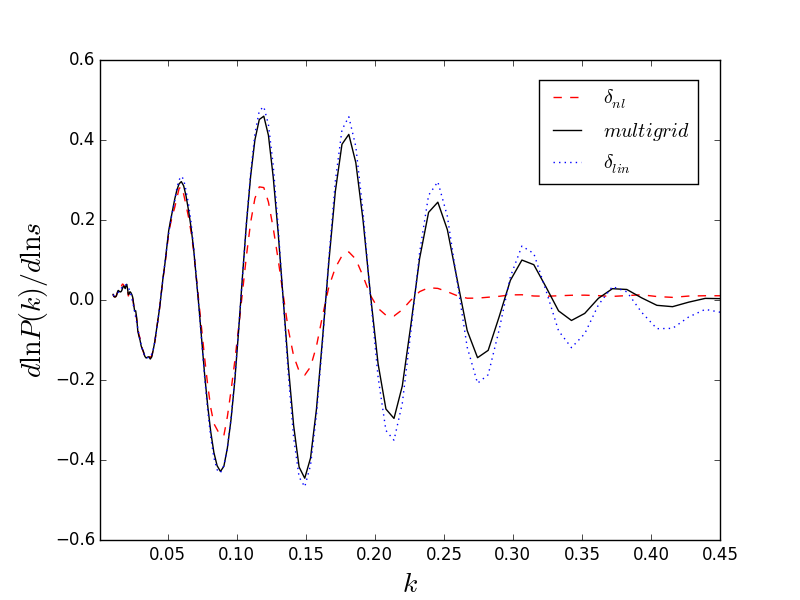
\includegraphics[width=3.4in]{Figures/dlnpk_dlns.png}

}
  \frame{
    \frametitle{FoM}
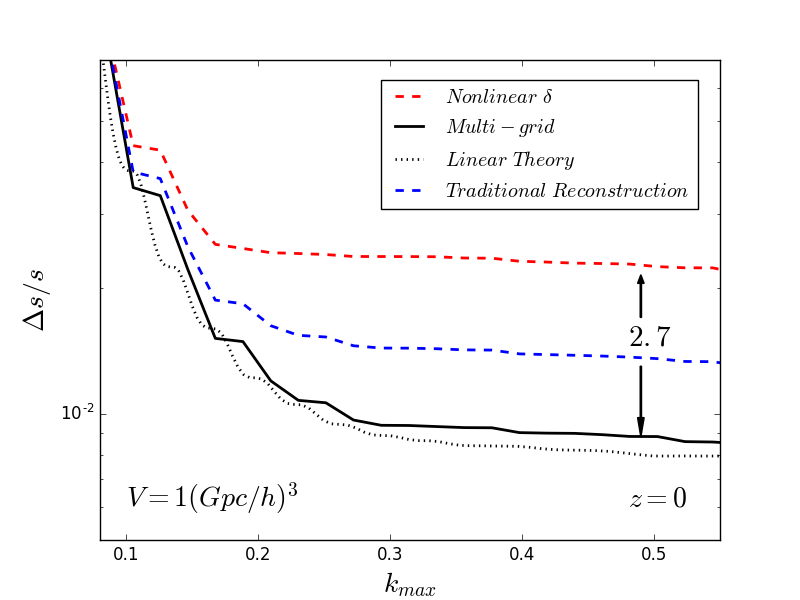
\includegraphics[width=3.4in]{Figures/bao_err_norm4_intp_logy.png}

}
  \frame{
    \frametitle{Halos}
\vspace{-4in}\hspace{-0.5in}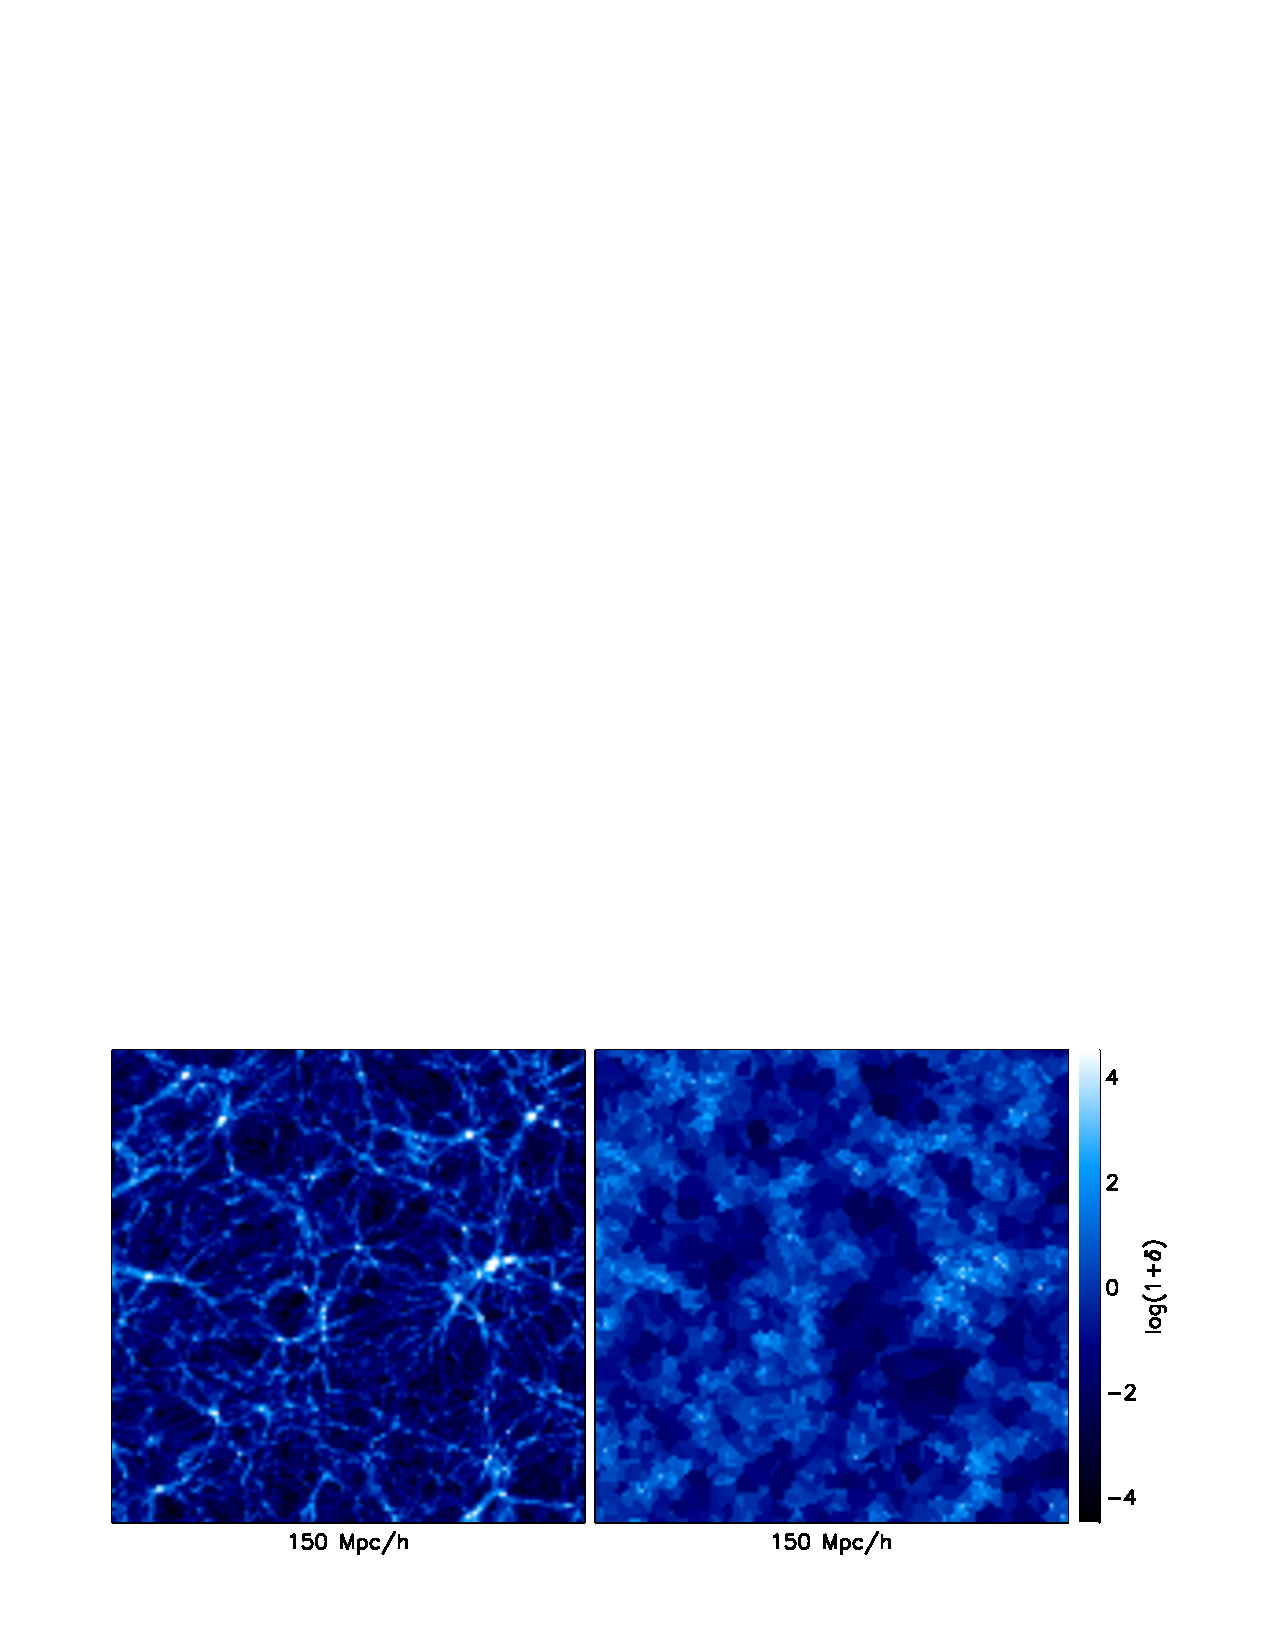
\includegraphics[width=5.0in]{Figures/map_both_150.pdf}

Voronoi tiling, Yu et al (2016, in prep)
}
  \frame{
    \frametitle{Halos}
\vspace{-0.5in}\hspace{-0.9in}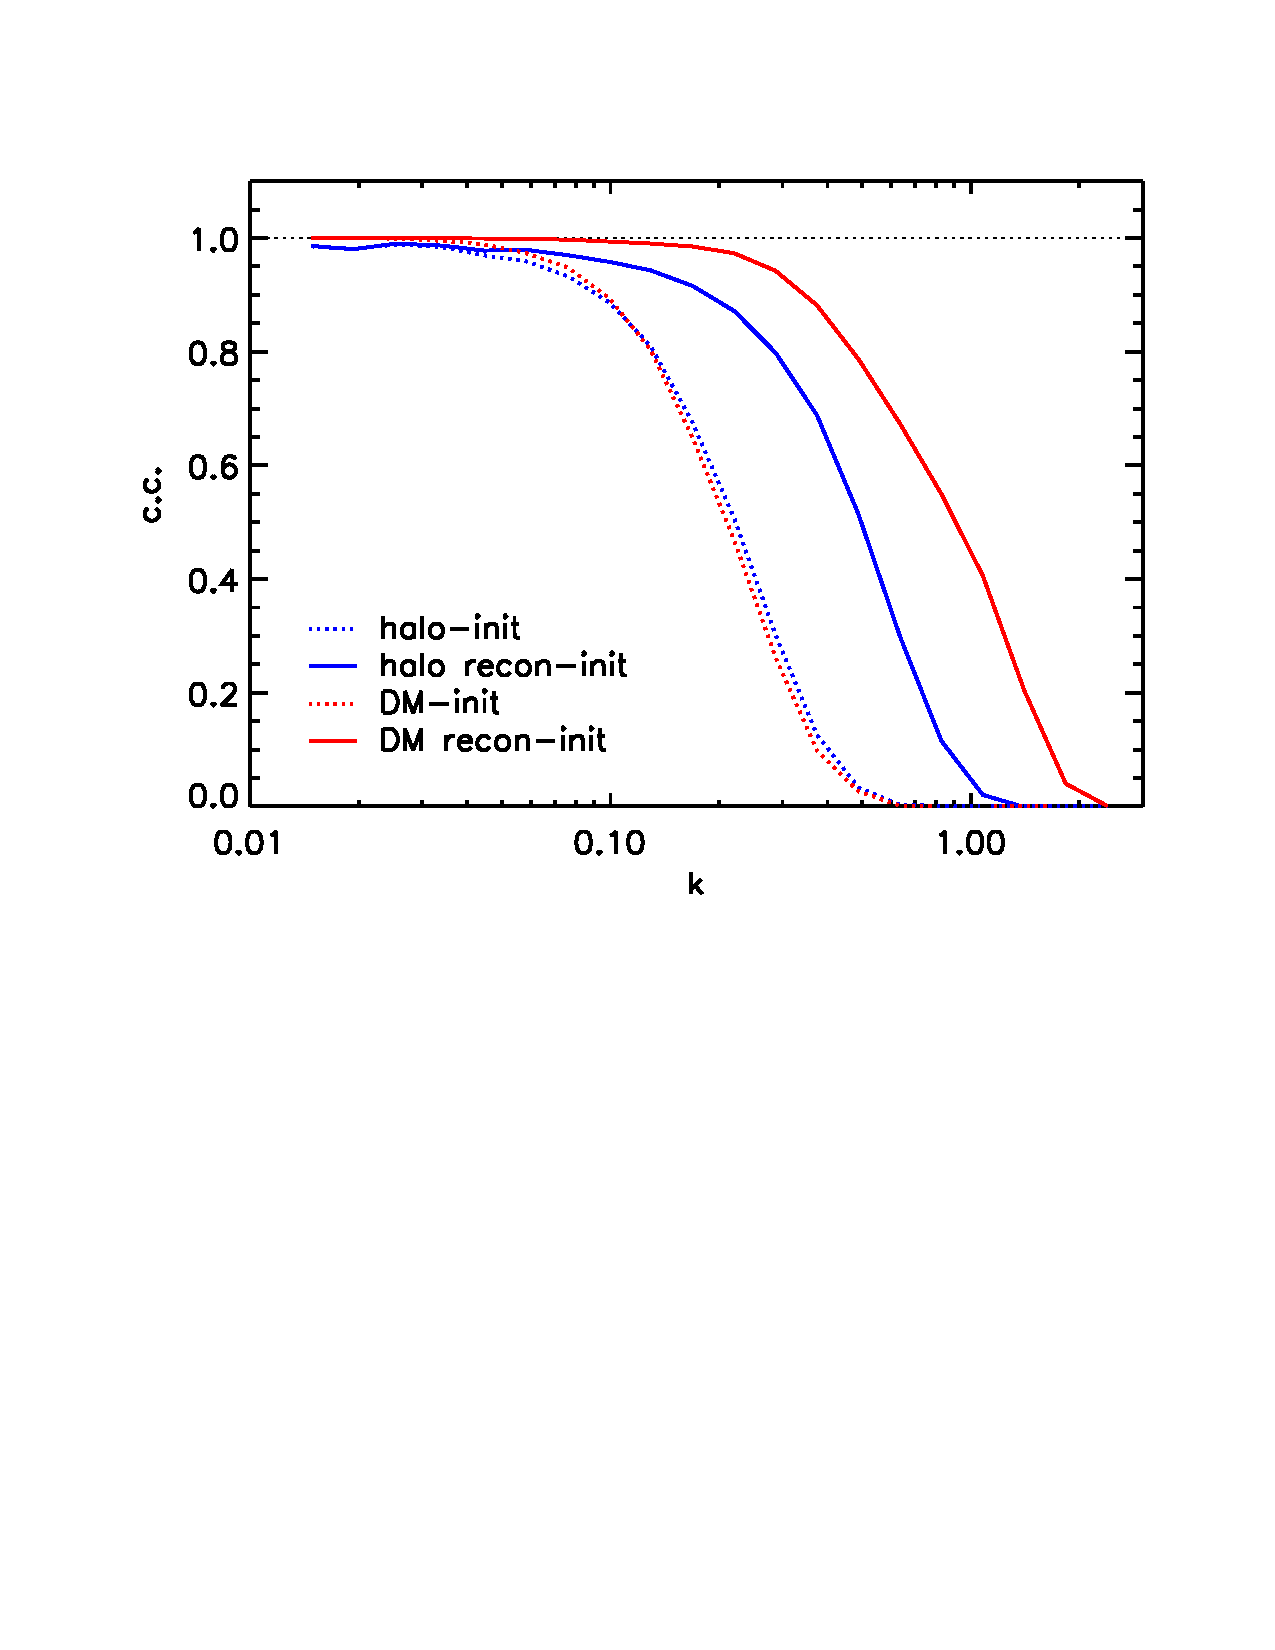
\includegraphics[width=5.0in]{Figures/halocc.pdf}
}

  \frame{
\vspace{-0.5in}
    \frametitle{low z, low noise, 21cm Surveys}
    \begin{itemize}
        \item tunable: Parkes, Tianlai, BINGO
        \item Highjacking: Apertif, GMRT, ASKAP, SKA
     \end{itemize}
  }

  \frame{
\vspace{-0.5in}
    \frametitle{Science applications}
    \begin{itemize}
        \item BAO: maximize leverage from low-z where dark energy dominates
        \item neutrino wake dipole
        \item RSD
     \end{itemize}
  }


\frame{
\vspace{-0.5in}
    \frametitle{Conclusions}
    \begin{itemize}
      \item Non-linear forward evolution: Neutrinos, halos, differential effects
      \item Non-linear backward mapping: bijiective potential isomass coordinates
      \item most precise non-parametric reconstruction mechanism to
          date
          \item computationally straightforward, mass coordinate
            similar to Lagrangian
        \item well suited for low shot noise low z BAO surveys,
          i.e. intensity mapping
     \end{itemize}
  }


\end{document}
